C is the grandad of most of the languages we use today. It's so good that people still use it to create the glorious Linux operating system. So, let's C what it can do!
\\
\\
\textbf{Additional Notes}\\
CHammond made some decent notes on most of this stuff if you want a quick but thorough overview of the module. Check them out on Google Drive if you have access, here: \url{https://docs.google.com/document/d/1t2VUYKYipdOwf7I22OtLSfnoMIe7KPTwmSjbXqMY5FI/edit}

\section{Basics}
C is an \gls{imperative} language, which means that you write programs by saying "do this!" then "do that!". Things get a little more complex than that when you're dealing with bigger programs (Linux kernel, anyone?) but essentially that's what it's about. Here's a quick rundown of things you can do.

\subsection{Literals}
Simply just the value. Using a literal is known as hard-coding as it cannot be changed when the program is running.

\subsection{Variables}
\Glspl{variable} are like, super important. They are the bread and butter of imperative programming, they are ways of storing values so that you can use them again or manipulate them however you desire. Let's look at a few different variable types and how you can define them. I'll also point out here that comments (notes you can add to the code that have no effect on the running) look like \texttt{/* this */} or like \texttt{// this}.
\begin{lstlisting}[language=C]
// Integers (whole numbers)
int someNumber = 42; // yer standard integer, 16 bits in size.
short yolo = 256; // a smaller integer.
char hiya = 25; // a very small integer, range of -127 to +127 makes it awesome for text characters.
long bigNum = 5484198; // For when you want to store biiiig numbers.

// Floating point numbers (numbers with decimal points)
float someNum = 3.4;  // single-precision, 32-bits.
double preciseNum = 3.232365;  // double-precision (durr)

bool amIRetakingTheYear = true;  // true or false, you need stdbool.h though.
\end{lstlisting}

Hey look at that, you can write C! To define a variable, you add the type you want in front of the name you're going to give it. You can then, if you want, assign it a value with the assignment (\texttt{=}) operator, or just leave it. To then access that variable or its value again, you only need its name.

\subsection{Simple Operators}
\Glspl{operator} are built-in mathsy things you can perform on variables. Here's a few you can do:
\subsubsection{Assignment}
Sets the value of a variable.
\begin{lstlisting}[language=C]
    lecturesMissed = 5;
\end{lstlisting}

\subsubsection{Addition}
Adds two numbers together. You can also just add a number on by combining this with the assingment operator.
\begin{lstlisting}[language=C]
    someStupidExample = 4 + 8; // is now 12.
    someStupidExample += 5;  // someStupidExample = 12 + 5 = 17.
\end{lstlisting}

\subsubsection{Subtraction}
Works \textbf{exactly the same} as addition, just with a minus (\texttt{-}) sign instead of a plus sign. Yes, this is starting to bore me now.

\subsubsection{Increment and Decrement}
You can add or subtract a single value with these. You have the choice of applying them before (prefix) or after (suffix). Check this:
\begin{lstlisting}[language=C]
    int some_num = 10;
    some_num++;  // some_num is now 11
    ++some_num;  // some_num is now 12
    some_num--;  // some_num is now 11
\end{lstlisting}

But why do you get the two separate ways of incrementing or decrementing numbers? It's because, when used in an expression, the prefix operator will use the new value in the expression, whereas the postfix will not. Let's see an example because my explanation is kinda bad.
\begin{lstlisting}[language=C]
    int i = 10;
    int k = ++i; // i = 10 + 1 = 11, THEN k = i = 11;
    int k = i++; // k = i = 11, THEN i = 11 + 1 = 12;
\end{lstlisting}
This is the cause of both misery and joy in my opinion. Use it at your own risk.

\subsubsection{Multiplication}
Again, works just like addition but with an asterisk (\texttt{*}).
\begin{lstlisting}[language=C]
    imBored = 5 * 12;  // is now 60.
\end{lstlisting}

\subsubsection{Division}
Hey, guess what? It works in EXACTLY THE SAME WAY. Honestly, I should be getting money for this. But what I will point out is that dividing an integer by an integer returns the whole part of a result, not rounded.
\begin{lstlisting}[language=C]
    int x = 5;
    int y = 2;
    x = x / y;  // x is now 2.
\end{lstlisting}

\subsubsection{Modulo}
It's very possible to get the remainder of dividing integers in C, you must use the modulo or remainder operator.
\begin{lstlisting}[language=C]
    ex = 5 % 2;  // 1, 5/2 is 2.5 or 2 with 1 left over
\end{lstlisting}

\subsubsection{Pointer (De)reference}
Woah there friend, you may need to slow down!

\subsection{Order Of Operations}
Pretty much 100\% confirmed as the first question in the exam. Like in real world maths, operators in C follow a 'precedence', e.g. some are always performed before others. This is known as order of operations, or operator precedence. It goes like this:
\begin{itemize}
    \item \textbf{1 (first)} - postfix increment/decrement, brackets etc.
    \item \textbf{2} - prefix increment/decrement, pointer stuff
    \item \textbf{3} - multiplication, division, modulo
    \item \textbf{4} - addition, subtraction
    \item \text{...} - a bunch of stuff that may not be so important right now.
\end{itemize}
Thanks, \url{http://en.cppreference.com/w/c/language/operator_precedence}.

\subsection{Arrays}
An array is a list of variables for which each have its own index. Basically, when you make your array, you get a big chunk of memory where you can store $n$ number of values... so naturally you can't change its size since that would be a shambles. But rather than try to explain memory voodoo to you, I'll leave that for later and just show you an example of how arrays work.

You define an array similarly to variables, except you're also providing a size.
\begin{lstlisting}[language=C]
    int someList[30];

    // let's give a list values!
    int anotherList[5] = {1, 3, 5, 6, 8};
\end{lstlisting}

It's probably best to think of arrays as like pigeon holes, where the number on the box is how you can refer to it.

\begin{figure}[h]
    \centering
    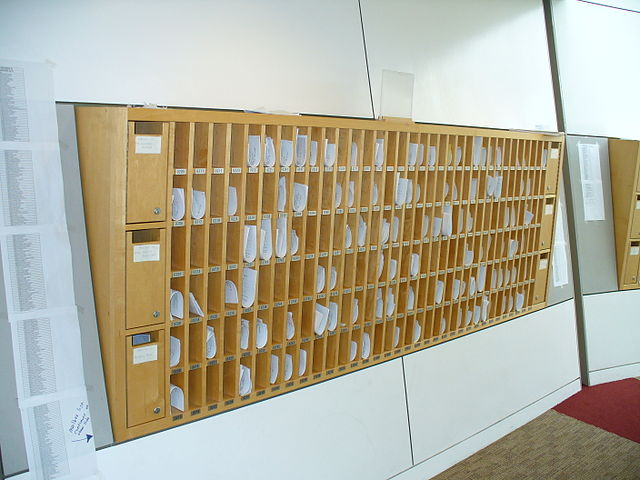
\includegraphics[width=0.5\textwidth]{pigeonhole}
    \caption{A pigeon hole. By "Stacalusa" on Wikipedia.}
\end{figure}

You can reference an item in the array just like any other variable, you just type \texttt{myArray[x]}, where \texttt{x} represents the index of the item (arrays count from 0 though, so beware!).

Since you can have arrays of any type (as long as each item has the same type as each other), you can actually have arrays of arrays, or 2-d arrays. They are simply defined like so:
\begin{lstlisting}[language=C]
    int some_2d_array[3][3] = {
        {1, 2, 3},
        {4, 5, 6],
        {7, 8, 9}
    };

    some_2d_array[1][2] = 4;
\end{lstlisting}

Oh oops, maybe I should point out at the same time that text is represented in C using \glspl{string}, which are quite literally an array of characters. Here's the difference though. You can define \gls{constant} strings (value doesn't change), by using this funky pointer notation (it will be explained later): \texttt{char *my\_string = "Dat boi";} They can also be represented with your standard ol' \texttt{char meme[10]} or whatever. Another difference is that strings have a hidden character at the end to say that the string is finished, called a 'null' character. It's represented as \texttt{\textbackslash0} and literally serves no other purpose.

\subsection{Call functions}
C comes with a bunch of \glspl{functions} which are blocks of code which do things. Some functions take in values and some return values, which makes them really handy for not writing the same damn piece of code a million times over. Most of them require you to import the related code \gls{library} to your program. You can do this like so, at the beginning of your file:

\begin{centering}
    \texttt{#include <stdlib.h>} - include a built-in library called "stdlib".\\
    \texttt{#include "mylib.h"} - include a library that is stored in the same directory which is called "mylib.h".\\
    \texttt{#include "libs/somelib.h"} - include a library that is stored in a directory called "libs".
\end{centering}

There's a couple of neat ones that you won't go wrong with remembering. They may come back when you least expect it!
\begin{itemize}
    \item \textbf{stdlib.h} - the 'standard' library which contains things like memory allocation, and value conversion (based \texttt{atoi()}, thank you).
    \item \textbf{stdio.h} - input/output library. Expect things like printing to console (\texttt{printf()}) as well as reading, along with file stuff too.
    \item \textbf{string.h} - helpful string library, which contains a bunch of helper functions such as comparing strings (\texttt{strcmp()}) and so on.
    \item \textbf{stdbool.h} - allows you to use the \texttt{bool} type, which is just true/false.
    \item \textbf{math.h} - this will save your butt, as well as containing mathsy things like trigonometry functions, you also get some neat constants like \texttt{M\_PI} which gives you Pi. Awesome!
\end{itemize}

\subsection{User-Defined Functions}
So, you want to make your own functions, huh? Very well. Functions are defined with, in order: the return variable type, the function name, as well as its \glspl{parameter} (if any), followed by the content of the function. Let's look at an example, we'll call it matt, and it will take an integer, add 5, and return it.
\begin{lstlisting}[language=C]
    int matt(int input) {
        input += 5;
        return input;
    }
\end{lstlisting}

That wasn't too bad was it? Note the "return" keyword. What this does is that it returns whatever you put after it. In this case, it's returning the value of \texttt{input}. This doesn't have to be a variable; if you had a function called \texttt{give\_me\_lemon} for instance, you could always have \texttt{return "lemon";} Also note that for each parameter, you need to provide its type. Very important.

Every program in C must have a main function, which returns either an \texttt{int} or \texttt{void}. Void is a magic keyword that means, "this function does not return anything". The main function is the entry point, the way in, to your program. Set things up there, I recommend.

\subsection{If Statements And Logic}
Maybe there's some code you don't want to run all the time. If statements are your solution!
\begin{lstlisting}[language=C]
    if (logical_statement) {
        do_something();
    }
    else if (another_statement) {
        do_something_else();
    }
    else {
        give_up();
    }
\end{lstlisting}

It's pretty self-explanatory. If the logical statement holds true, then the code in the first block is used. If it is false, then the else statement is used. In this case above, the else statement contains another if-else statement, testing for another statement. So only if both logical statements are false, then the last code block will be used.

But what is a logical statement? It's an expression that returns true or false. For this, we can use \glspl{logicalop} to take variables and reduce them to something boolean. Let's explore them.

\subsubsection{Equals Operator}
The equals operator takes two variables, literals, functions or whatever of the same type and returns true if they are equal, and false if not. You type \texttt{==} to use it.
\begin{lstlisting}[language=C]
    int my_num = 5;
    if (my_num == 5) {
        // this will execute as my_num is equal to 5.
    }
\end{lstlisting}

Don't use this for strings! You should use the \texttt{strcmp()} function from stdlib.h for that.

\subsubsection{Not Equals Operator}
Does the exact opposite of what equals does, funnily enough. This is represented with \texttt{!=}. Do you really need an example for this?

\subsubsection{Less Than (Or Equal To) Operator}
Given two values, you can test if one is less than the other. You can use \texttt{<} for just that, or you can be bold and use \texttt{<=} to additionally make the statement true if the two values are equal. Superb!
\begin{lstlisting}[language=C]
    int my_score = 10;
    if (my_score < 30) {
        give_up(); // this will be executed.
    }
\end{lstlisting}

\subsubsection{Greater Than (Or Equal To) Operator}
Uhm, it's the opposite of the less than operator.

\subsubsection{Logical Not Operator}
This will invert a logical statement or boolean value given to it, represented just by the \texttt{!} character.
\begin{lstlisting}[language=C]
    if (!true) {
        // this will NEVER run since !true becomes false.
        // Why you would write code like this, I don't know.
        // But if you ever do, I recommend you take a cold hard
        // look at your code and wonder just why.
    }
\end{lstlisting}

\subsubsection{Logical Or Operator}
This takes two logical statements and will return true if \textit{either} of them are true. You use the \texttt{||} (two pipes) characters for this.
\begin{lstlisting}[language=C]
    int gimme_five() {
        return 5;
    }

    int x = 10;
    if ((x == 10) || (x == gimme_five())) {
        // x == 10 so this is true. Never mind that x is not equal
        // to the output of gimme_five()
    }
\end{lstlisting}

\subsubsection{Logical And Operator}
This returns true only if both statements are true. This is represented with the \texttt{\&\&} characters.
\begin{lstlisting}[language=C]
    bool do_you_need_this(int score, bool failed) {
        if ( (score > 30) && !failed) {
            return false;
        }
        else {
            return true;
        }
    }
\end{lstlisting}

So nice one, you can do that now!

\section{Intermediate Programming}
Oh, so you think you're a big guy now? You've finished the basics stuff and you want something more, something a little more complex? Well you've come to the right place buster, it's time for some intermediate C.

\subsection{Loops}
Loops are great because you can repeat stuff many times without having to write it out each time. You can repeat stuff without having to write it out each time, which is great.

\subsubsection{While Loop}
While loops are run infinitely while the logical statement is true. So you gotta be careful otherwise it can run forever if your logical statement doesn't change. Unless you want that to happen, you maverick you.
\begin{lstlisting}[language=C]
    int i = 0;
    while (i < 10) {
        printf("Hello");
    }
    // prints out HelloHelloHelloHelloHelloHelloHelloHelloHelloHello
\end{lstlisting}

If you are a true renegade, you can put the logical statement at the end to create a "do-while" loop. This is then checked at the \textit{end} of each loop, which means that the loop is guaranteed to run at least once.
\begin{lstlisting}[language=C]
    int i = 0;
    do {
        printf("Hello");
    } while(i > 1);
    // prints out Hello
\end{lstlisting}

\subsubsection{For Loop}
Oh, now you've done it. So you're not content enough with just a while loop; you want something that looks more badass. So I give you the for loop. You have statement to run before the loop, a state to check at the beginning of each loop, and a statement to run at the end of each loop. It looks a bit like this.
\begin{lstlisting}[language=C]
    for (inital_thing(); test_this(); at_the_end_of_each_loop();) {
        do_something();
    }

    // In practice:
    int i;
    for (i = 0; i < 10; i++) {
        printf("%d",i);
    }
    // Prints "12345678910"
\end{lstlisting}

You get me? You have me got? Good.

\subsection{Bait And Switch}
The switch statement is a kinda neat way of testing for many different values without having some massive if-else if-else if and so on. You specify a "switch", and then test for values, which \textbf{must} be literals, as well as a default. Each 'case' as they are known must end with a \texttt{break} so that the code exits the switch statement rather than go down to the next one.
\begin{lstlisting}[language=C]
    char input = get_some_input();

    switch (input) {
        case 'a': menu_option_1();
                  break;
        case 'b': printf("2B or not 2B");
                  break;
        default:  printf("Nice work, you mug.");
                  break;
    }
\end{lstlisting}

\subsection{A Big Hand For Our Cast}
Type casting is a handy way of converting certain variable types to another. It's useful for converting floats to integers, for example.
\begin{lstlisting}[language=C]
    double x = 4.5;
    int y = (int) x;
    // y is now 4.
\end{lstlisting}

\subsection{A Couple Of Pointers}
So this is the one that makes people cry. And honestly, pointers shouldn't if you treat them right! A pointer is kinda what you'd imagine it to be, a type of variable that stores a memory address, so it literally "points" to an actual variable. When you create a variable normally, e.g. \texttt{int why = 10}, you're asking what's called the "heap" memory for some space to store an integer. It'll get the memory address of that space it's been allocated, so that the program can then write into that space.

What is a memory address you ask? Memory on a computer is divided into loads of little sections of a certain size, and they are numbered so that that space can be remembered. Think of each space like a car parking space, and the address is the number painted on the floor in front of the space, and the data is the car... I'm not sure where I'm going with this analogy.

The cool thing with C is, you can very much fiddle with the memory addresses to your liking (the memory given to your program by the operating system, that is). But as a wise Uncle Ben once said, with great power comes great responsibility. And you really do have the potential to mess up your program with pointers (although your computer is safe).

General pointer stuff is baked into the C language, however you may need to use the \texttt{stdlib.h} library to access some of the memory functions.

\subsubsection{Get Thine Address}
The \texttt{\&} operator gets the address of a variable. No man, nothing to do with the logical AND operator! You put it in front of a variable name to return its address.
\begin{lstlisting}[language=C]
    int x = 101;
    printf("%d\n", &x); // this prints out 0x4328db or some such thing.
\end{lstlisting}

\subsubsection{Pointer Type}
A pointer type is completely different to its variable bretheren. It just stores a pointer and nothing else, although the type of pointer determines just how big the memory space that it's pointing at is. A pointer type is defined using the asterisk, in the form \texttt{<type> *<var\_name>}.
\begin{lstlisting}[language=C]
    int some_val = 346;
    int *my_ptr = &some_val;
    // my_ptr now points at the location of some_val
\end{lstlisting}

\subsubsection{Dereference the pointer}
You have a pointer which is nice, but it'd be rather swish if you could get the value it's pointing at right? Hence you need the dereference operator. You have to use the asterisk before the variable's name, and bam there you go.
\begin{lstlisting}[language=C]
    int some_val = 645;
    int *my_ptr = &some_val;
    some_val += 10;
    printf("my_ptr looks at %d\n", *my_ptr);
    // prints out "my_ptr looks at 655"
    // ARE YOU A MAGICIAN
\end{lstlisting}

The cool thing about this is that you can use pointers to pass in variables to functions rather than just their values, so you can change them in-situ. They also have their uses in arrays. Say whaaaat? You heard me, arrays use pointers already. The index format (\texttt{array[10]}) is just syntactic sugar for \texttt{*(array + 10)}, which means get the address of array, and add 10 to it, then return whatever's stored there (array items are stored in adjacent memory locations, fortunately). This is why you may see arrays passed into functions or what have you as something like \texttt{int *some\_array} if the length isn't known, or how strings are passed as \texttt{char *my\_string}.

\subsubsection{Pass By Reference}
Whenever you use a variable in a parameter for a function, you're giving the function the value of the variable rather than the variable itself. But you can change this if you wish, by passing the variable pointer instead. Let's look at this interesting example.
\begin{lstlisting}[language=C]
void add_five(int *num) {
    *num += 5;
}

int main() {
    int x = 10;
    add_five(&x); // address of x is passed into add_five since it needs a pointer.
    // The value of x is now 15.
}
\end{lstlisting}
Hey, that ain't too hard!

\subsection{Rollin' In The Heap}
So it's all well and good doing that stuff above with pointers, but you can also use the blighters to create and destroy variables in memory as you like. Introducing the heap, a section of memory that's dedicated \textit{just} for this purpose.
\subsubsection{Get Memory From The heap}
\begin{lstlisting}[language=C]
    #include <stdlib.h>

    int *my_ptr = (int *) malloc (sizeof (int));
\end{lstlisting}
What you've got here, is that a new int pointer is created, which points at some new allocated memory. The \texttt{malloc()} literally means "Memory ALLOCate", and accepts a size as its parameter; in this case we're using the \texttt{sizeof()} function to get the size of an int type. Finally, we use a type cast to make the pointer into an int pointer. But why stop there? Let's make an array using heap memory, since that's a thing right?
\begin{lstlisting}[language=C]
    #include <stdlib.h>

    int arr_size = 10;
    float *array = (float *) malloc (arr_size * sizeof(float));

    array[0] = 10.4; // first element
    *(array + 2) = -23.653; // third element (counts from 0 right?)
\end{lstlisting}

\subsubsection{Destroy Memory From The Heap}
You're done with your data and you now want to release that piece of memory back to the heap to be used again. This is good because if you never release to the heap, you can run out of heap memory and you will cry.
\begin{lstlisting}[language=C]
    #include <stdlib.h>

    int * p = (int *) malloc( sizeof (int) );
    *p = 10;
    // blah blah blah
    free(p);
    // the address of p can now be overwritten
\end{lstlisting}

\subsection{In N' Out}
Programs are rather more handy when a user is able to interact with it. It does bring you some extra problems though (the user is an idiot), but that's well outside the scope of this course. Let's do some output. You'll need to include the \texttt{stdio.h} library for these functions.

\subsubsection{printf}
\texttt{printf()} lets you write out (or 'print' as the oldies call it) text to what's known as STDOUT. Normally this is just the screen, so let's go with that. You give printf a format string, followed by variables you want to output.
\begin{lstlisting}[language=C]
    int x = 10;
    printf("The pointless value of x is %d\n", x);
    // prints out "The pointless value of x is 10"
\end{lstlisting}

\subsubsection{Format Strings}
Let's talk more about the format strings and why they look scary. You've got your standard text, as well as conversion characters and special characters. These are the common special characters:
\begin{itemize}
    \item \textbf{\textbackslash~n} - Newline character, use this to start a new line.
    \item \textbf{\textbackslash~r} - Return character, if you're on Windows then this will probably be of use to you.
    \item \textbf{\textbackslash~0} - Null character, this is at the end of every string.
    \item \textbf{\textbackslash~t} - tab character, if you want to align your text all neat and that.
\end{itemize}

Want an actual backslash? Just use two backslashes next to each other.

Now, these are the conversion characters:
\begin{itemize}
    \item \textbf{\%~s} - String.
    \item \textbf{\%~d} - Integer.
    \item \textbf{\%~f} - Floating point number.
    \item \textbf{\%~c} - Character.
\end{itemize}
You can also combine these with a number to represent a certain number of characters to display. So, \texttt{\%4d} would be a nice way of displaying currency (probably). Want to use an actual percentage sign? Just use it twice again!

\subsubsection{scanf}
\texttt{scanf()} is one way of getting user input. It's the safest way of getting user text from
